\documentclass[10pt]{exam}
\usepackage[phy]{template-for-exam}
\usepackage{enumitem,multirow,tikz,multicol}

\title{Car Lab \#2 (\emph{Accelerated Motion})}
\author{Rohrbach}
\date{\today}

\begin{document}
\maketitle

\vspace{-1em}
\section*{Procedure:}
  \begin{enumerate}[label=\alph*),topsep=0pt,itemsep=-1ex,partopsep=1ex,parsep=1ex]
    \item 
      Find a spot on the hallway for your group and mark every 25 cm for 125 cm
    \item 
      Set the car at 25 cm and pull it back to the starting line.
    \item 
      Measure the time it takes the car to go 0.25 m
    \item
      Repeat for 0.50, 0.75, 1.00, and 1.25 meters.  Make sure you pull the car back from 25 cm each time.
    \item
      Repeat three times
    \item 
      For experiment \#2, make an additional mark (``charge point'') 1.0 meters behind the starting line and a second mark (``release point'') 25 cm behind that.
    \item 
      For experiment \#2, pull the car back from ``charge point'' to ``release point,'' but don't start the timer until the car gets to ``start.''  We are trying to capture the part of the motion where the car is slowing down.
  \end{enumerate}

  \tikzstyle{marker}=[fill=orange,draw=orange]
  \tikzstyle{charge}=[fill=purple,draw=purple]
  \tikzstyle{arrow}=[->,ultra thick, purple]
  \tikzstyle{lab}=[below]
  \tikzstyle{dim}=[<->]
  \tikzstyle{pullarrow}=[anchor=south west, text width=6cm]
  \def\markwidth{.02}
  \def\abovesp{0.3}
  \tikzset{x=5cm}

  \noindent
  \begin{tikzpicture}
      
    \draw[charge] (-1,0) rectangle ++(\markwidth,-1) 
      ++(-0.5*\markwidth,0) node[lab] {charge} 
      +(0,-0.4) node[lab] {point}
      ++(0,1) ++(0,\abovesp) coordinate (pull);

    \draw[marker] (-1.25,0) rectangle ++(\markwidth,-1) 
      ++(-0.5*\markwidth,0) node[lab] {release}
      +(0,-0.4) node[lab] {point}
      ++(0,1) ++(0,\abovesp) coordinate (release);

    \draw[marker] (0,0) rectangle ++(\markwidth,-1) 
      ++(-0.5*\markwidth,0) node[lab] (start) {start};

    \draw[charge] (0.25,0) rectangle ++(\markwidth,-1) 
        ++(-0.5*\markwidth,0) node[lab] {0.25 m};

    \foreach \x in {1.75, 1.50, 1.25, 1.00, 0.75, 0.50}{
      \draw[marker] (\x,0) rectangle ++(\markwidth,-1) 
        ++(-0.5*\markwidth,0) node[lab] {\x{} m};
    }

    \draw[dim] (-0.95,-0.5) -- (-0.05,-0.5)
      node[fill=white,midway] {\footnotesize 1.0 m};
    \draw[dim] (-1.05,-0.5) -- (-1.2,-0.5)
      node[fill=white,midway,rotate=90] {\footnotesize 25 cm};

    \draw[arrow] (pull) -- (release) 
      node[anchor=south west, text width=6cm] 
      {\emph{Experiment \#2: Pull car from ``charge point'' to ``release point''.}};

    \draw[arrow] (0.25,-1.5) -- ++(-0.25,0) 
      node[anchor=north west, text width=6cm] 
      {\emph{Experiment \#1: Pull car from 25 cm to ``start''.}};

  \end{tikzpicture}

  \vspace{-2em}

\section*{Data}

  \def\cw{6em}


  \renewcommand{\arraystretch}{1.3}

  \paragraph{Experiment \#1:} Accelerating Motion

    \begin{tabular}
      {|*{3}{>{\centering\arraybackslash}m{\cw}|}|*{2}{>{\centering\arraybackslash}m{\cw}|}}
      \hline
      Trial \#1 Time (s) & 
      Trial \#2 Time (s) & 
      Trial \#3 Time (s) & 
      Average Time (s)  & Displacement (m) \\
      \hline
      0.00 & 0.00 & 0.00 & 0.00 & 0.00\\
      \hline
      &&&& 0.25\\
      \hline
      &&&& 0.50\\
      \hline
      &&&& 0.75\\
      \hline
      &&&& 1.00\\
      \hline
      &&&& 1.25\\
      \hline
    \end{tabular}

  \paragraph{Experiment \#2:} Decelerating Motion

    \begin{tabular}
      {|*{3}{>{\centering\arraybackslash}m{\cw}|}|*{2}{>{\centering\arraybackslash}m{\cw}|}}
      \hline
      Trial \#1 Time (s) & 
      Trial \#2 Time (s) & 
      Trial \#3 Time (s) & 
      Average Time (s)  & Displacement (m) \\
      \hline
      0.00 & 0.00 & 0.00 & 0.00 & 0.00\\
      \hline
      &&&& 0.25\\
      \hline
      &&&& 0.50\\
      \hline
      &&&& 0.75\\
      \hline
      &&&& 1.00\\
      \hline
      &&&& 1.25\\
      \hline
      &&&& 1.50\\
      \hline
      &&&& 1.75\\
      \hline
    \end{tabular}

  
  \section*{Graph} 
    Make a graph on Desmos.
    
\begin{multicols}{2}

  \begin{enumerate}[label=\alph*),topsep=0pt,itemsep=-1ex,partopsep=1ex,parsep=1ex]
    \item \label{table} Start by making a table by clicking the “+” icon at the top left.  You will need to create two separate tables.
    \item \label{wrench} Make sure to label the axes using the wrench icon at the right.
    \item \label{zoom} Zoom out so that you can see the whole graph and so that it fills the page.  You can do this using the ``Zoom Fit'' option, but be careful that your fit does not cut off one of the graphs
    \item \label{linear} Create best fit lines for each graph using the ``Linear Regression'' tool
  \end{enumerate}

    \begin{tikzpicture}[x=1cm,y=1cm]
      \node[anchor=north west] at (0,0) 
        {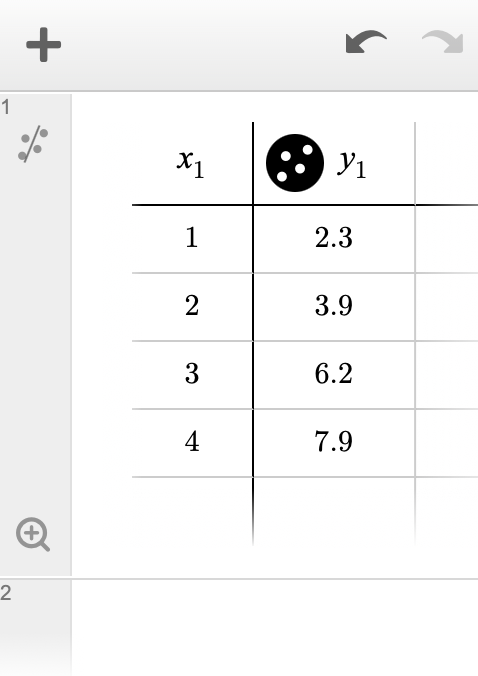
\includegraphics[width=3cm]{desmos1}};


      \node[anchor=north west] at (3.5,0) 
        {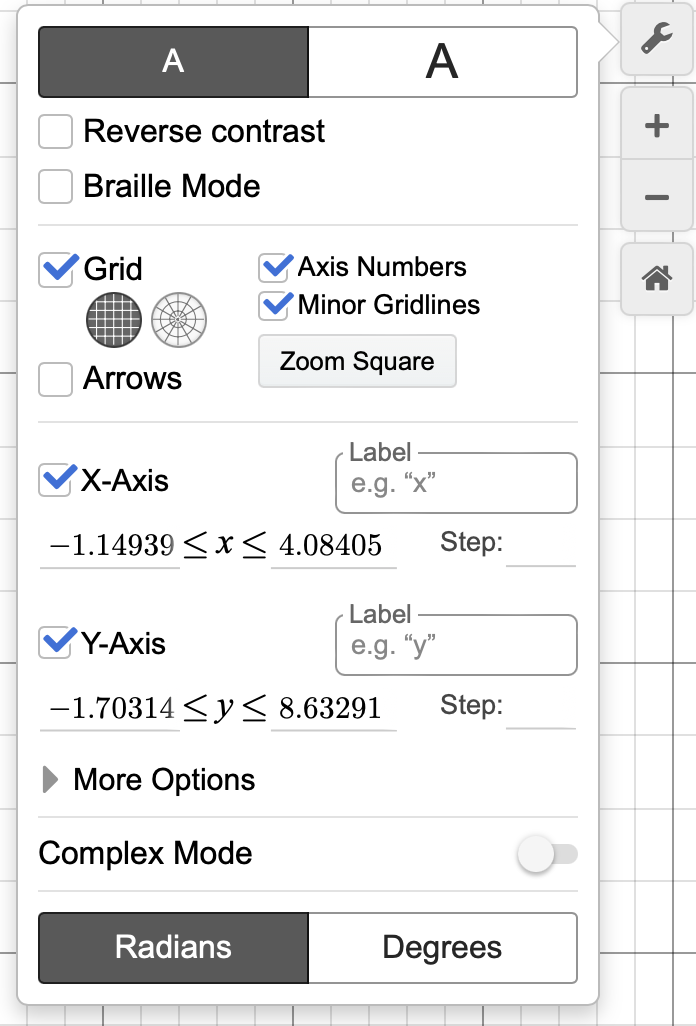
\includegraphics[width=3.5cm]{desmos2}};

          \draw (2,0) 
        node[fill=red!20,rounded corners] (table)
        {\ref{table} Create a table};
      \draw[red] (0.4,-.4) coordinate (a) circle (0.3);
      \draw[<-,red,very thick] (a) +(0.3,0) -- (table.south);

      \node[fill=blue!20,rounded corners] at (2.5,-1.5) (linear) {\ref{linear} Linear Regression};
      \draw[blue] (0.3,-1) coordinate (a) circle (0.3);
      \draw[<-,blue,very thick] (a) +(0.3,0) -- (linear.north);

      \node[fill=green!20,rounded corners] at (2,-2.5) (zoom) {\ref{zoom} Zoom Fit};
      \draw[green, ultra thick] (0.3,-3.5) coordinate (a) circle (0.3);
      \draw[<-,green,very thick] (a) +(0.3,0) -- (zoom.west);

      \node[fill=orange!20,rounded corners] at (4.5,-0.5) (wrench) {\ref{wrench} Axis Labels};
      \draw[orange, ultra thick] (6.9,-.3) coordinate (a) circle (0.3);
      \draw[<-,orange,very thick] (a) +(-0.3,0) -- (wrench.east);

      \draw[->,orange,very thick] (wrench.south) -- (5.2,-2.3);

      \draw[orange, ultra thick, rounded corners] (3.8,-2.3) rectangle ++(2.8,-0.5);
      \draw[orange, ultra thick, rounded corners] (3.8,-3.1) rectangle ++(2.8,-0.5);
    \end{tikzpicture}


\end{multicols}


\section*{Analysis}

\begin{questions}

  \question
    Try making a best fit line.  How well does this best-fit line represent your data?  Give a reason why a line is not good for this data.
    \vs

  \question
    Instead make of a linear regression, use the drop-down menu on Desmos to change to \textbf{\it ``Quadratic''}.  Write down the formulas for each of the best fit curves

    \begin{multicols}{2}
    

    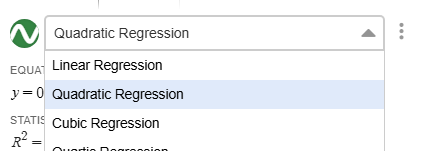
\includegraphics[width=7.5cm]{desmos4}
    
    \vspace{1em}

    Best Fit Curve \#1 (Accelerated Motion):

    \vspace{3em}

    Best Fit Curve \#2 (Decelerated Motion):

    \vspace*{3em}

  \end{multicols}

    \emph{After you've done this, make sure to submit your graph on Schoology}.
      
  \question
    Explain why the shape of each graph makes sense.  
    \vs

  
  \question
    Your graphs are not perfect.  What were some aspects that limited the accuracy of our graphs and our precision?  What could be done to mitigate these in future experiments?
    \vs
  
  


\end{questions}

\end{document}